% Hello, world

Since the fall of 2022, I've been teaching intro stats and I've been very particular about my graphs. According to my college ethics professor, the experience of beauty is a human good and statistics is not.\footnote{Shoutout to the late Alfonso G\'{o}mez-Lobo.} That doesn’t provide a good prioritization for developing an intro stats syllabus, but as an instructor, I've at least tried to make my slides and notes a kind of beautiful. Watching a student pinch to zoom on her iPad without a particular graph pixelating or otherwise revealing any defect was a beautiful moment. 

I make all of the figures for my class materials in Python. Working in Python offers the advantage of, well, working in Python. We are able to mix statistical functions from Python in our code, so we gain more precision than is available from anything hand-drawn (whether on pencil and paper or by dragging a cursor). We can also create high quality images in a vector format like PDF or SVG, meaning we can zoom without the image quality degrading. 

It's true that you might achieve the same goals using languages like R or Ti$k$z. Indeed, for probability trees, I still use Ti$k$z. Otherwise, I offer no apology for choosing Python. In this chapter, I include a few common applications that arise in statistics. 


\begin{center}
    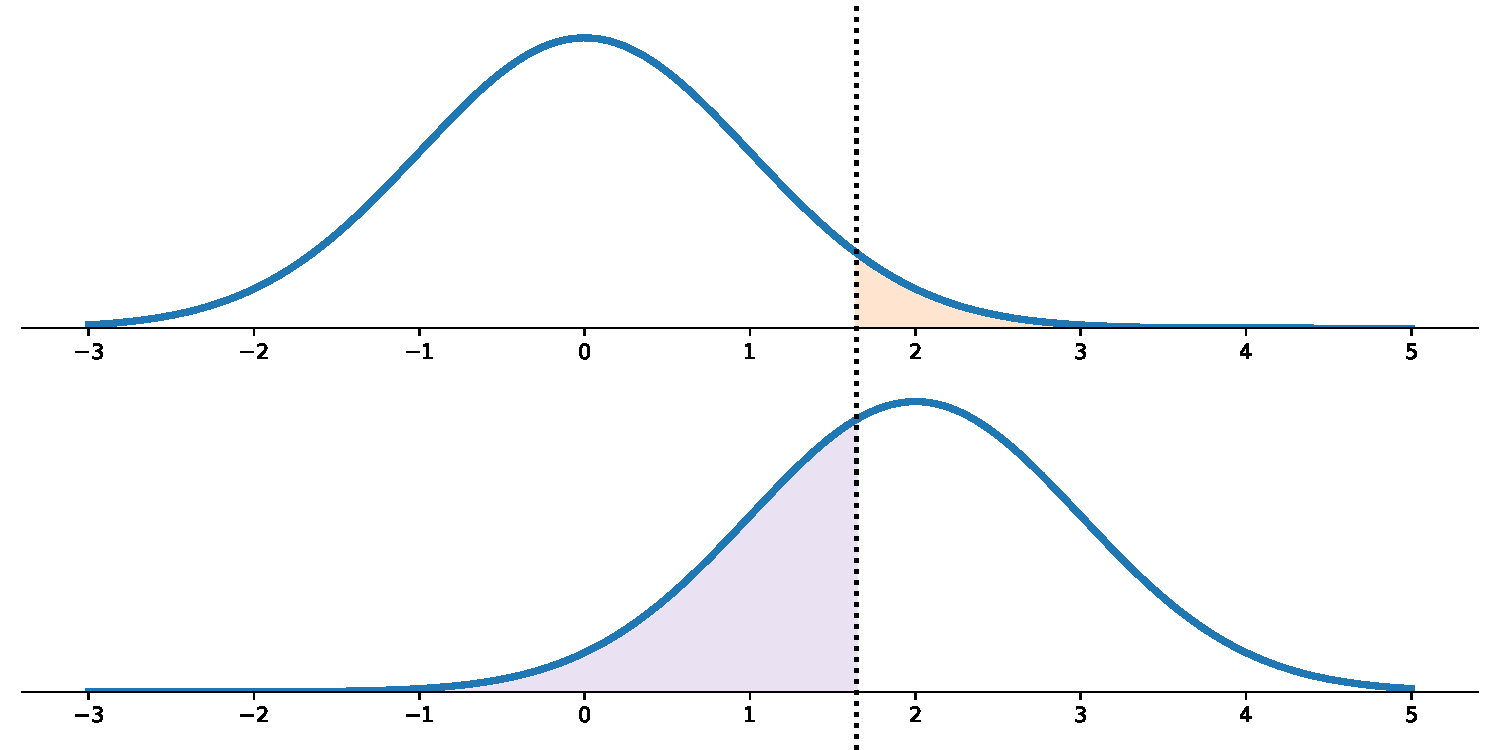
\includegraphics[width = 0.95\textwidth]{figures/specialplots/errors-stacked.pdf}
\end{center}


\section{Probability Diagrams}

%Venn diagrams are a standard illustration for concepts like the intersection of two sets. 
Below, we produce Venn diagrams to consider set operations for two sets, $A$ and $B$. These sets are outlined as circles, either by plotting the outline or by using the Circle artist object. The result of the set operation will be filled with gray. This can be tricky because I insist that the circle outlines (the Artist object's edge) are always visible, meaning we have to be mindful of how one circle overlapping another could obscure the other's outline. 

First, we plot $A$ and $B$, filling only $A$. $A$ and $B$ are Circle objects and I plot $B$ second so that it is in front of $A$. This means that the outline of $B$ is not lost underneath $A$. We want the opposite from the fill color of $B$---we do not want it to overlap $A$. To prevent this, $B$ is filled with \code{facecolor = (1, 1, 1, 0)}, which is the RGBA color for white (RGB 1,1,1) and an alpha or opacity of 0\%, leaving it transparent. We could also have used an alpha parameter, but this would apply to both the \code{facecolor} and \code{edgecolor} arguments, which we want to treat separately. 

\pyfile{event-A.py}

\begin{center}
    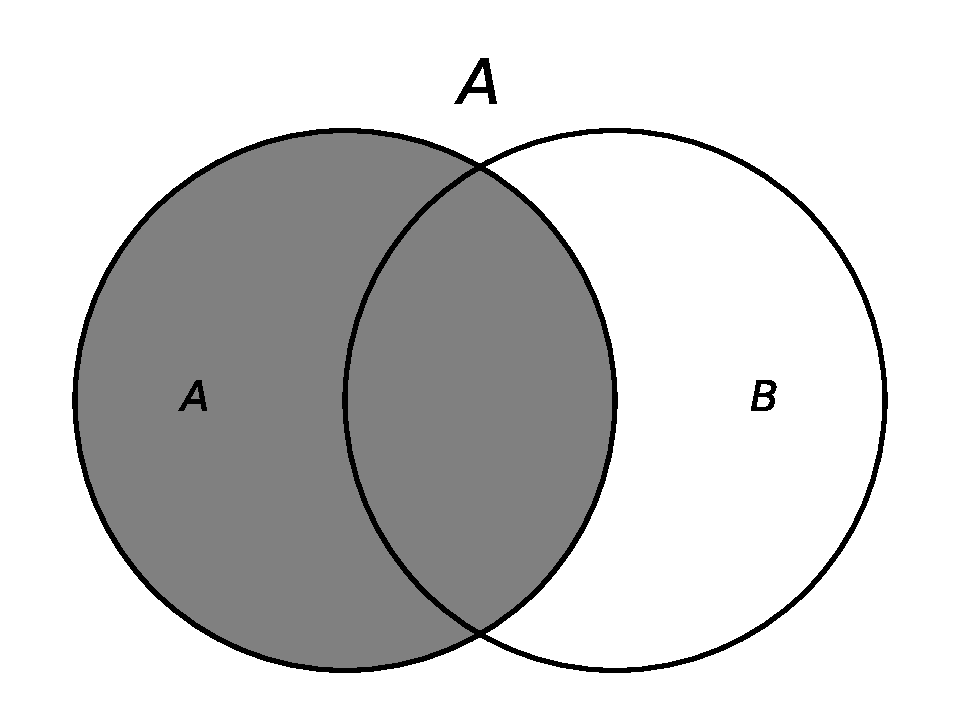
\includegraphics[width = 0.7\textwidth]{figures/specialplots/event-A.pdf}
\end{center}

Next, we consider the union of $A$ and $B$. This presents a similar challenge in not having the fill of one circle cover the outline of the other circle. First, we create two Circle objects, filled gray and with a black outline.  If we stopped there, we would have a visible overlap. To recover the outline of $A$, we add a third circle with a black outline but a transparent fill. 

\pyfile{union.py}

\begin{center}
    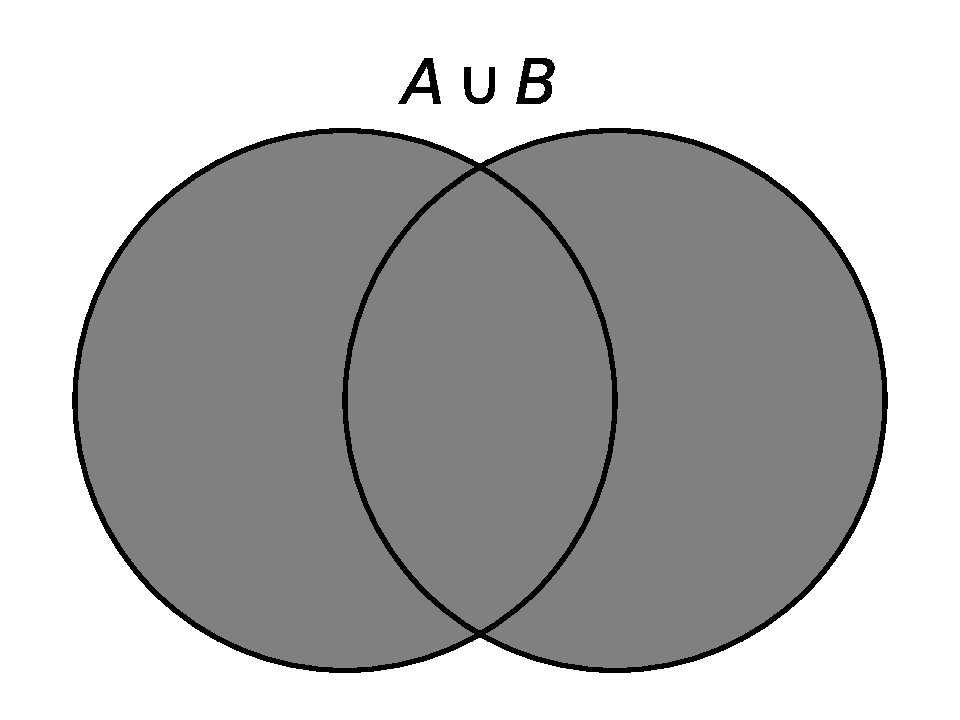
\includegraphics[width = 0.7\textwidth]{figures/specialplots/union.pdf}
\end{center}


To plot the intersection of $A$ and $B$, we abandon Circle objects for the \code{plot()} and \code{fill_between()} Axes methods. Filling the intersection is done in two pieces. 

\pyfile{intersection.py}

\begin{center}
    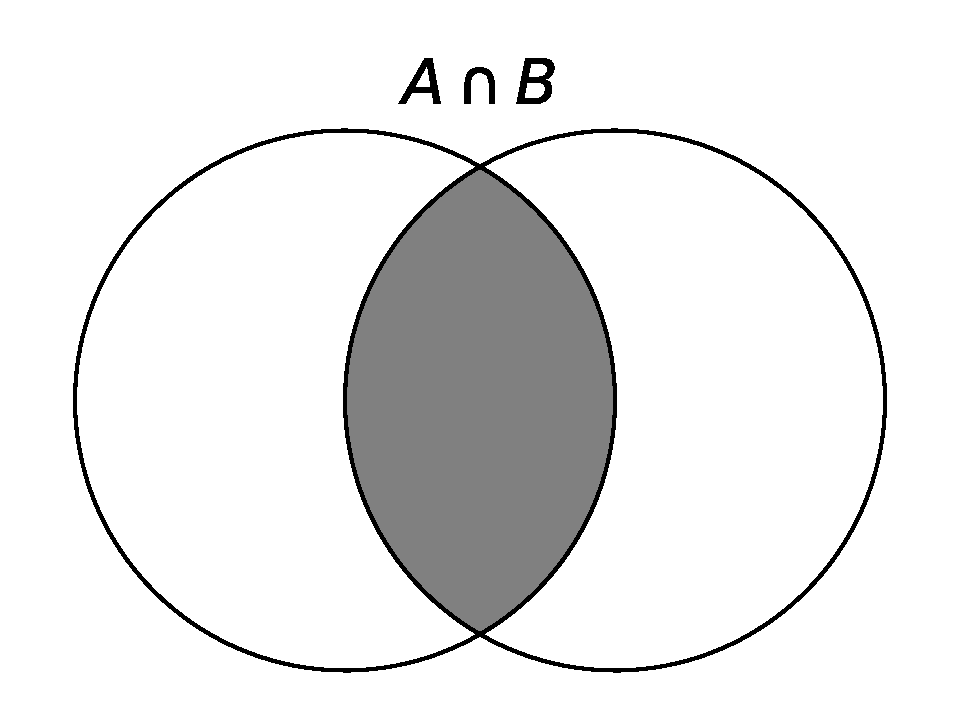
\includegraphics[width = 0.7\textwidth]{figures/specialplots/intersection.pdf}
\end{center}

Finally, we plot $A \cap B^C$ or $A\setminus B$. For this, we again need a third transparent circle. We allow a white-filled $B$ to cover $A \cap B$, essentially removing the fill from that region. Then, we use the Circle \code{left_circle_helper} to restore the outline of $A$. 

\pyfile{A-minus-B.py}

\begin{center}
    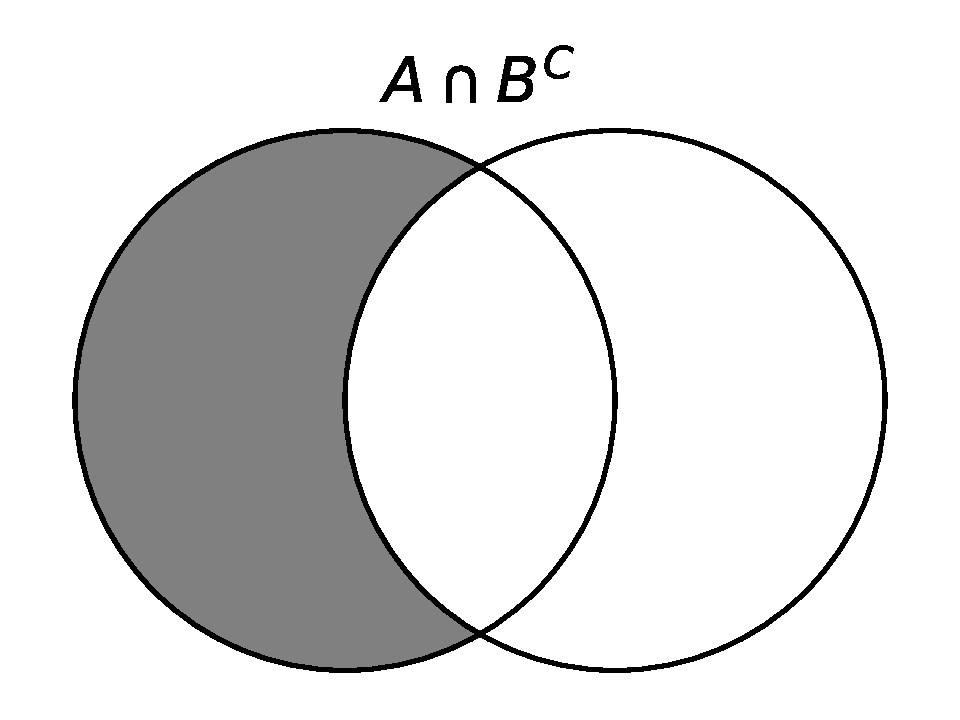
\includegraphics[width = 0.7\textwidth]{figures/specialplots/A-minus-B.pdf}
\end{center}


\section{Distributions}


We use the \code{hist()} Axes method to create a histogram. Beautifying the plot is only a matter of modifying the background elements, like the spines and labels, and then choosing the right number of bins and colors for the histogram. A histogram includes Patch objects, meaning we can specify both an \code{edgecolor} and \code{facecolor}. Below, we create a histogram using the defaults. 

\pyfile{default-hist.py}

\begin{center}
    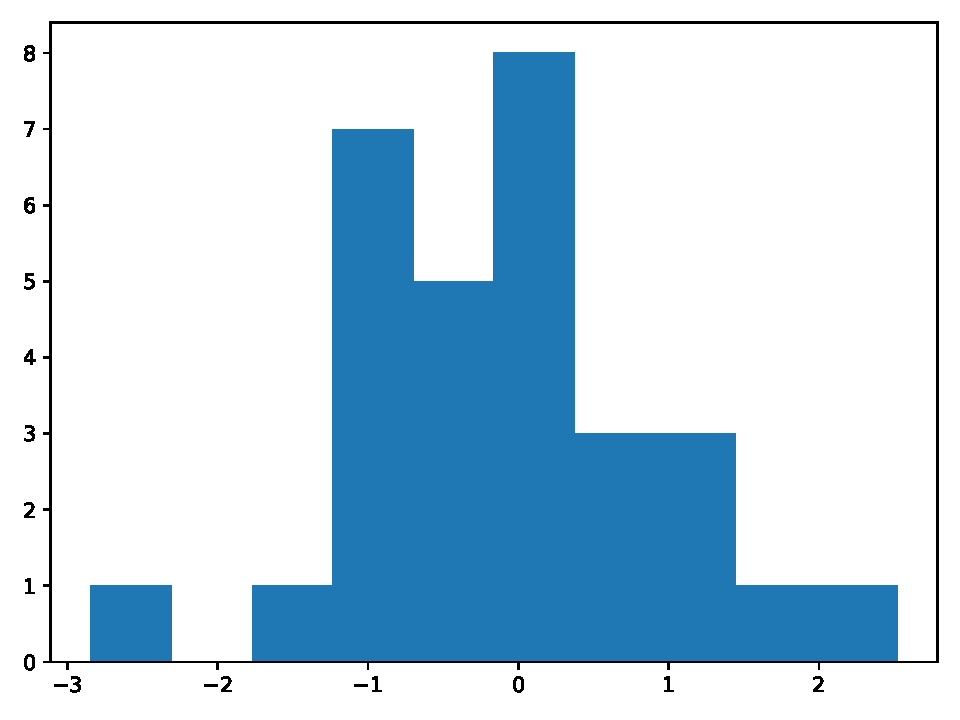
\includegraphics[width = 0.7\textwidth]{figures/specialplots/default-hist.pdf}
\end{center}

When you are only interested in the shape of the data, you will find the $y$-axis information unimportant. Accordingly, we'll remove the $y$-axis to (repeat after me) reduce clutter. 

\pyfile{clean-hist.py}

\begin{center}
    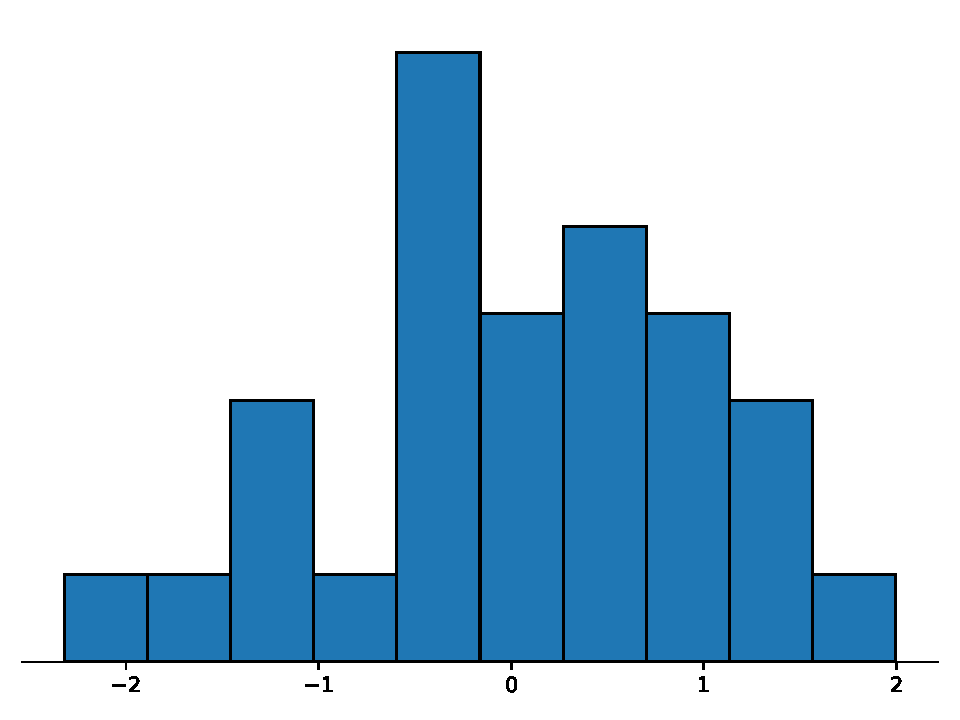
\includegraphics[width = 0.7\textwidth]{figures/specialplots/clean-hist.pdf}
\end{center}

The last modification considered is the simple use of the \code{bins} parameter to adjust the number of bins in the histogram. 

\pyfile{bins-hist.py}

\begin{center}
    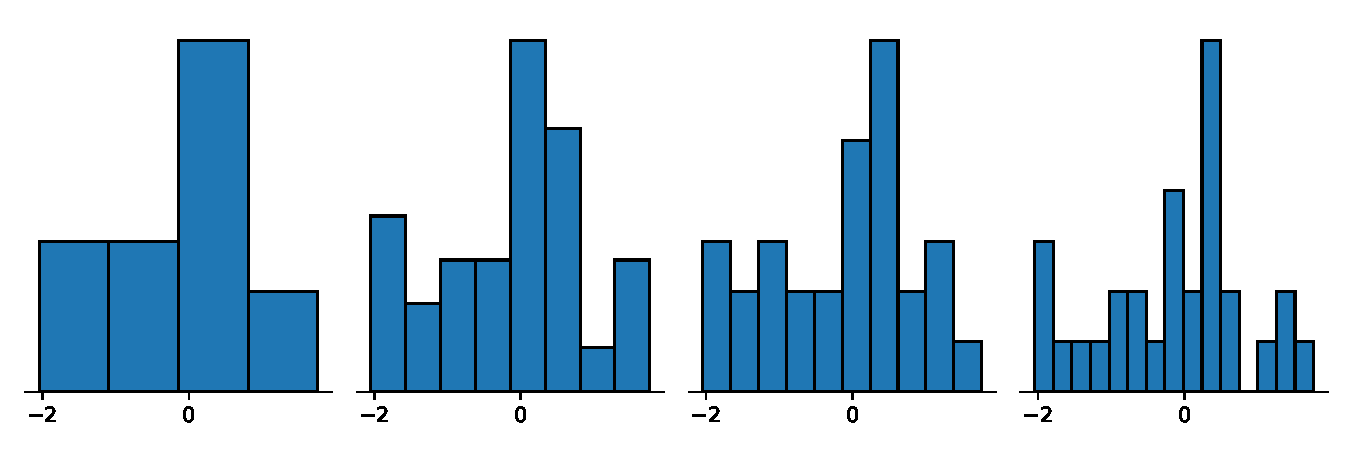
\includegraphics[width = 0.7\textwidth]{figures/specialplots/bins-hist.pdf}
\end{center}

Next, density plots can be produced the SciPy package and its statistics module, which has been imported already with \code{import scipy.stats as stats}. Below is a simple plot for a normal distribution. 

\pyfile{normal-pdf.py}

\begin{center}
    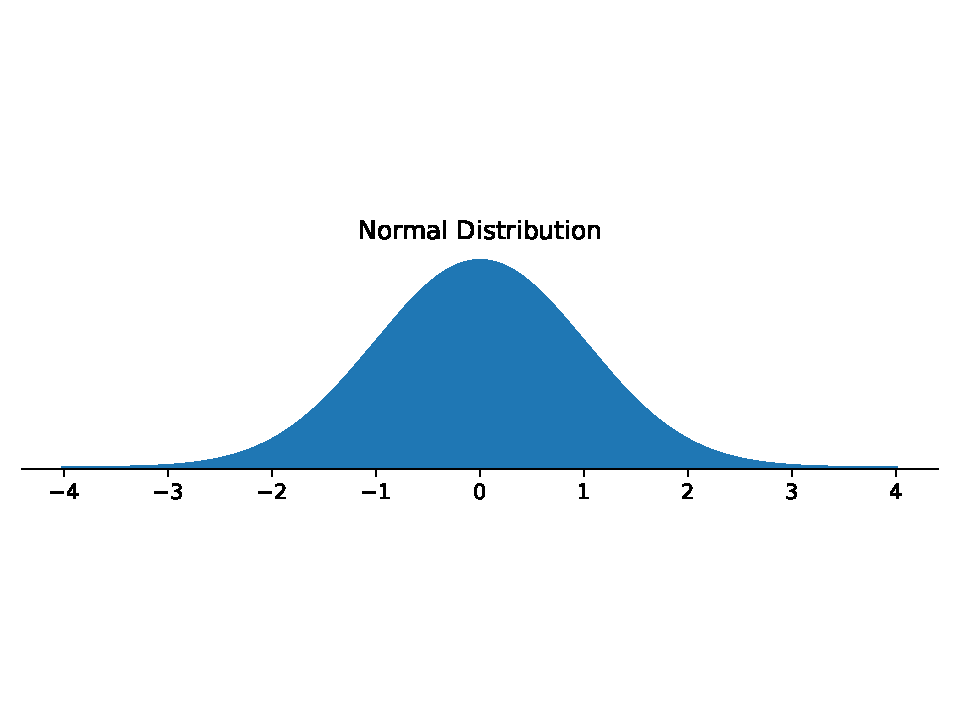
\includegraphics[width = 0.7\textwidth]{figures/specialplots/normal-pdf.pdf}
\end{center}
